\usetikzlibrary{calc}
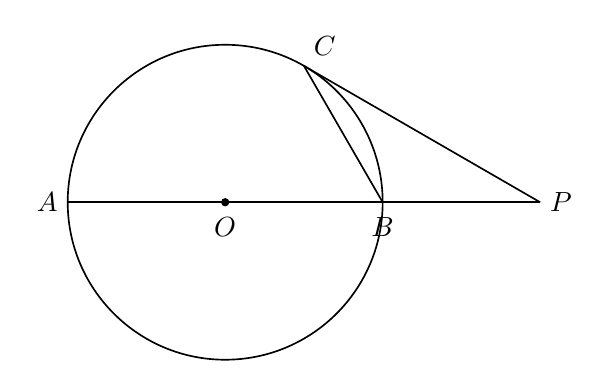
\begin{tikzpicture}[x=1cm,y=1cm,line width=.6pt,font=\normalsize]
\coordinate (O) at (0,0);
\coordinate (A) at (-2,0);
\coordinate (B) at (2,0);
\coordinate (P) at (4,0);
\coordinate (C) at (1,1.7320508076);
\draw (O) circle[radius=2cm];
\draw (A)--(P);
\draw (P)--(C);
\draw (B)--(C);
\fill (O) circle (1.5pt);
\node[left] at (A) {$A$};
\node[below=2pt] at (O) {$O$};
\node[below=2pt] at (B) {$B$};
\node[right] at (P) {$P$};
\node[above right] at (C) {$C$};
\end{tikzpicture}
